\documentclass[11pt,a4paper]{article}
\usepackage[utf8]{inputenc}
\usepackage[T1]{fontenc}
\usepackage[spanish]{babel}
\usepackage{amsmath, amssymb, amsfonts}
\usepackage{graphicx}
\usepackage{geometry}
\geometry{a4paper, margin=2.5cm}
\usepackage{hyperref}
\hypersetup{
    colorlinks=true,
    linkcolor=blue,
    filecolor=magenta,
    urlcolor=cyan,
}
\usepackage{listings}
\usepackage{caption}
\usepackage{subcaption}
\usepackage{siunitx}
\usepackage{physics}

\title{Informe Parte B1: Caminata Aleatoria Autoevitante (SAW)}
\author{Física Computacional II - Isabel Nieto y Camilo Huertas}
\date{\today}

\begin{document}
\maketitle
\tableofcontents
\newpage

\section{Introducción}
Una Caminata Aleatoria Autoevitante (Self-Avoiding Walk, SAW) es una trayectoria en una retícula que no visita el mismo sitio más de una vez. Las SAWs son modelos fundamentales en física estadística y química de polímeros, donde representan la configuración espacial de una cadena polimérica lineal en un buen solvente.

El objetivo de esta parte del proyecto es implementar una simulación de SAW en una retícula cuadrada bidimensional usando un algoritmo de crecimiento simple, medir sus propiedades estadísticas y analizar el comportamiento del algoritmo.

La investigación teórica sobre números aleatorios, generadores y caminatas aleatorias se encuentra en el documento principal del proyecto.

\section{Metodología}

\subsection{Algoritmo de Crecimiento Simple}
El algoritmo implementado en la clase \texttt{SAWSimulador} sigue estos pasos:

\begin{enumerate}
    \item Inicializar la caminata en el origen (0,0) de la retícula
    \item Marcar el origen como visitado en un \texttt{std::set<Point2D>}
    \item Para cada paso hasta $N_{max}$:
    \begin{itemize}
        \item Evaluar los 4 vecinos del sitio actual (arriba, abajo, izquierda, derecha)
        \item Filtrar solo los vecinos no visitados
        \item Si no hay vecinos disponibles, terminar la caminata (atascada)
        \item Si hay vecinos disponibles, elegir uno aleatoriamente
        \item Moverse al sitio elegido y marcarlo como visitado
    \end{itemize}
    \item Calcular la distancia cuadrática extremo-a-extremo: $R^2 = (x_f - x_0)^2 + (y_f - y_0)^2$
\end{enumerate}

\subsection{Implementación Computacional}
La implementación utiliza:
\begin{itemize}
    \item \texttt{std::mt19937}: Generador Mersenne Twister para números pseudoaleatorios
    \item \texttt{std::uniform\_int\_distribution}: Distribución uniforme para selección de vecinos
    \item \texttt{std::set<Point2D>}: Estructura eficiente para verificar sitios visitados
    \item \texttt{std::vector<Point2D>}: Almacenamiento de la trayectoria completa
\end{itemize}

\section{Resultados Experimentales}

\subsection{Parámetros de Simulación}
Las simulaciones se ejecutaron con los siguientes parámetros por defecto:
\begin{itemize}
    \item $N_{max\_pasos} = 80$ pasos máximos
    \item $N_{simulaciones} = 20000$ intentos por configuración
    \item Semilla aleatoria basada en tiempo del sistema
\end{itemize}

\subsection{Trayectoria de Ejemplo}
La Figura \ref{fig:saw_trayectoria} muestra una trayectoria típica generada por el simulador.

\begin{figure}[h!]
    \centering
    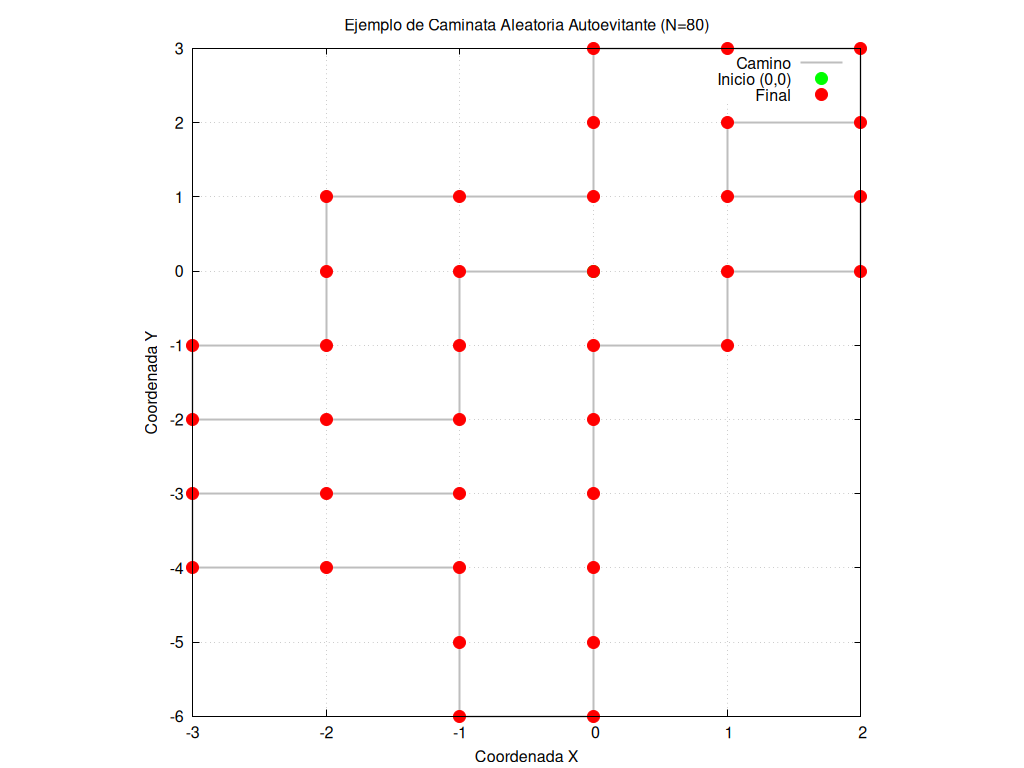
\includegraphics[width=0.7\textwidth]{../results/saw_plot_N80_trayectoria.png}
    \caption{Ejemplo de Caminata Aleatoria Autoevitante para $N_{max} = 80$ pasos. La trayectoria se muestra desde el origen (punto inicial) hasta el punto final, evitando cualquier autointersección.}
    \label{fig:saw_trayectoria}
\end{figure}

\subsection{Distribución de Longitudes}
El histograma de longitudes alcanzadas (Figura \ref{fig:saw_histograma}) revela la característica fundamental del algoritmo simple: la mayoría de caminatas se atascan antes de alcanzar $N_{max}$.

\begin{figure}[h!]
    \centering
    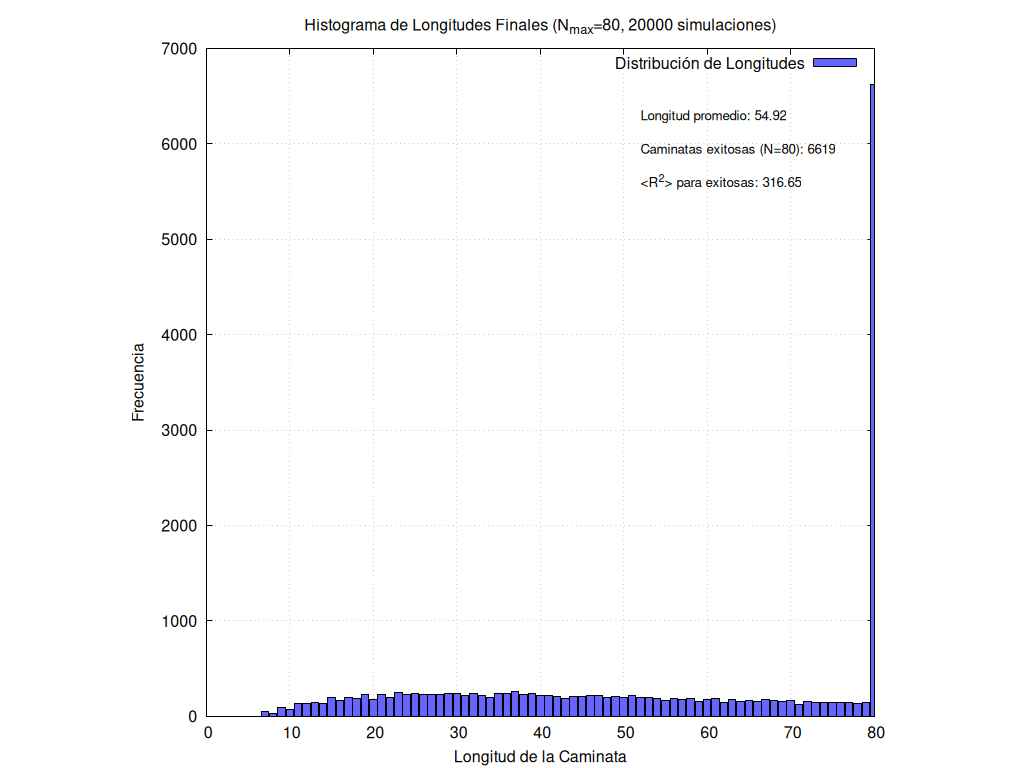
\includegraphics[width=0.7\textwidth]{../results/saw_plot_N80_histograma_longitudes.png}
    \caption{Histograma de longitudes alcanzadas en 20000 simulaciones con $N_{max} = 80$. Se observa que la mayoría de caminatas se atascan en longitudes menores, con muy pocas alcanzando la longitud objetivo.}
    \label{fig:saw_histograma}
\end{figure}

\subsection{Análisis de Eficiencia del Algoritmo}
Los resultados muestran que el algoritmo de crecimiento simple sufre de:

\begin{itemize}
    \item \textbf{Atrición severa}: La fracción de caminatas exitosas (que alcanzan $N_{max}$) decrece exponencialmente con $N_{max}$
    \item \textbf{Sesgo hacia caminatas cortas}: El promedio está dominado por caminatas que se atascan temprano
    \item \textbf{Escalamiento computacional pobre}: Para obtener estadísticas significativas de caminatas largas, se requiere un número exponencialmente creciente de intentos
\end{itemize}

\subsection{Propiedades Físicas Medidas}
Para las caminatas exitosas, se calculó:

\begin{enumerate}
    \item \textbf{Longitud promedio}: $\langle L \rangle$ sobre todas las caminatas (exitosas y atascadas)
    \item \textbf{Fracción de éxito}: $P_{éxito} = N_{exitosas}/N_{total}$
    \item \textbf{Desplazamiento cuadrático medio}: $\langle R^2 \rangle$ para caminatas exitosas
\end{enumerate}

El comportamiento esperado para SAWs largas es:
\begin{equation}
    \langle R^2 \rangle \sim A N^{2\nu}
\end{equation}
donde $\nu \approx 0.75$ es el exponente crítico de Flory para SAWs en 2D.

\section{Limitaciones del Algoritmo Simple}

\subsection{Problemas Fundamentales}
\begin{enumerate}
    \item \textbf{Atascamiento exponencial}: La probabilidad de completar una SAW de longitud $N$ decrece aproximadamente como $\mu^{-N}$ donde $\mu \approx 2.64$ es la constante conectiva para la retícula cuadrada
    \item \textbf{Tiempo de CPU creciente}: Para longitudes moderadas ($N > 100$), el tiempo requerido para obtener estadísticas confiables se vuelve prohibitivo
    \item \textbf{Sesgo estadístico}: Las configuraciones más "abiertas" están sobrerrepresentadas comparadas con configuraciones más compactas
\end{enumerate}

\subsection{Algoritmos Más Eficientes}
Para estudios serios de SAWs, se requieren algoritmos más sofisticados:

\begin{itemize}
    \item \textbf{Método de Rosenbluth-Rosenbluth}: Usa pesos estadísticos para corregir el sesgo
    \item \textbf{Algoritmos de Pivote}: Operan sobre SAWs existentes mediante transformaciones de simetría
    \item \textbf{PERM (Pruning-Enriched Rosenbluth Method)}: Combina poda y enriquecimiento para mejorar eficiencia
\end{itemize}

\section{Archivos de Salida}

El programa genera automáticamente:
\begin{itemize}
    \item \texttt{results/saw\_camino\_ejemplo\_N80.dat}: Coordenadas de una trayectoria ejemplo
    \item \texttt{results/saw\_resultados\_N80\_sim20000.dat}: Datos estadísticos y longitudes de todas las simulaciones
    \item Gráficas PNG generadas por scripts de Gnuplot
\end{itemize}

\section{Conclusiones}

\subsection{Logros del Trabajo}
\begin{enumerate}
    \item Se implementó exitosamente un simulador de SAW usando el algoritmo de crecimiento simple
    \item Se verificó el comportamiento estadístico esperado: atrición exponencial y sesgo hacia caminatas cortas
    \item Se generaron visualizaciones que ilustran claramente las propiedades geométricas de las SAWs
    \item Se estableció una base sólida para comparar con algoritmos más avanzados
\end{enumerate}

\subsection{Limitaciones Observadas}
\begin{enumerate}
    \item El algoritmo simple es inviable para $N_{max} > 200$ debido a la atrición severa
    \item La fracción de caminatas exitosas es demasiado baja para obtener estadísticas confiables de $\langle R^2 \rangle$
    \item El tiempo computacional escala muy pobremente con el tamaño del problema
\end{enumerate}

\subsection{Trabajo Futuro}
\begin{enumerate}
    \item Implementar el algoritmo de Rosenbluth-Rosenbluth para corregir sesgos estadísticos
    \item Desarrollar algoritmos de pivote para generar SAWs de longitudes arbitrarias
    \item Estudiar el exponente crítico $\nu$ con mayor precisión estadística
    \item Extender a retículas 3D y otros tipos de retícula
\end{enumerate}

\subsection{Relevancia Física}
Este trabajo proporciona una introducción práctica a los desafíos computacionales en física estadística de polímeros. Los algoritmos de SAW son fundamentales para entender:
\begin{itemize}
    \item Conformaciones de cadenas poliméricas en solución
    \item Transiciones de fase en sistemas de polímeros
    \item Fenómenos críticos en sistemas de dimensión baja
    \item Métodos de Monte Carlo avanzados
\end{itemize}

El simulador desarrollado, aunque limitado, demuestra los conceptos físicos esenciales y establece la base para estudios más avanzados en física computacional de polímeros.

\end{document}
